\documentclass[journal]{IEEEtran}

\usepackage{amsmath,amssymb,amsfonts}
\usepackage{algorithmic}
\usepackage{algorithm}
\usepackage{graphicx}
\usepackage{textcomp}
\usepackage{xcolor}
\usepackage{cite}
\usepackage{booktabs}
\usepackage{multirow}
\usepackage{url}
\usepackage{hyperref}
\usepackage{bm}
\usepackage{tikz}
\usepackage{stfloats}
\usetikzlibrary{arrows.meta, positioning, shapes.geometric, fit, calc, decorations.pathreplacing}

\graphicspath{{figures/}}

\begin{document}

\title{Learning Radar Waveforms: End-to-End Neural Generation via Differentiable Ambiguity Functions}

\author{Marc~Bara%
\thanks{M. Bara is with ESADE Business School, Barcelona, Spain (e-mail: marcoantonio.bara@esade.edu). ORCID: 0009-0005-1480-5760.}%
}

\markboth{IEEE Transactions on Aerospace and Electronic Systems}%
{Bara: Learning Radar Waveforms via Differentiable Ambiguity Functions}

\maketitle

% ==============================================================
\begin{abstract}
We present end-to-end neural radar waveform generation, enabled by a differentiable implementation of the ambiguity function compatible with automatic differentiation (AD) frameworks.
A neural network takes design parameters---such as trade-off weights between peak sidelobe level (PSL) and low probability of intercept (LPI)---as input and outputs optimized constant-modulus waveforms.
Training is performed by backpropagating through the differentiable ambiguity function, so that gradients flow from radar performance metrics directly into the network weights.
Once trained, the generator produces waveforms for any design specification in under one millisecond, replacing the 7--14 seconds required by iterative optimization per waveform.
We formulate the differentiable ambiguity function using parallelized FFT operations with proper Wirtinger derivative handling, achieving $O(N^2 \log N)$ complexity while maintaining mathematical equivalence to the standard periodic ambiguity function.
Experimental validation demonstrates that (i) optimizing the full 2D ambiguity function achieves 7.3~dB PSL improvement over 1D autocorrelation baselines and 2.2--3.0~dB over genetic algorithms, (ii) new constraints such as spectral masks can be added with zero gradient re-derivation, and (iii) the neural waveform generator produces waveforms within 0.3--1.6~dB of iterative methods at over 10{,}000$\times$ faster inference.
All experiments report mean $\pm$ standard deviation over multiple random seeds (5--20 depending on computational cost).
GPU benchmarks and open-source code are provided.
\end{abstract}

\begin{IEEEkeywords}
Radar waveform design, ambiguity function, automatic differentiation, neural networks, low probability of intercept, cognitive radar.
\end{IEEEkeywords}


% ==============================================================
\section{Introduction}
\label{sec:intro}

Radar waveform design is a cornerstone of modern remote sensing, with the ambiguity function~\cite{woodward1953probability, levanon2004radar} serving as the fundamental tool for characterizing range and Doppler resolution capabilities.
The ambiguity function $\chi(\tau, f_d)$ quantifies the matched filter response at delay~$\tau$ and Doppler shift~$f_d$, providing insight into sidelobe behavior, resolution performance, and overall waveform quality.
Real-world radar systems demand waveforms that simultaneously satisfy multiple conflicting objectives---low sidelobes, spectral constraints, low probability of intercept---making waveform design an inherently multi-objective optimization problem~\cite{blunt2016overview}.

Traditional approaches to this problem fall into three categories.
Metaheuristic methods such as genetic algorithms (GA) and particle swarm optimization (PSO) treat the ambiguity function as a black-box evaluation metric~\cite{kim2025modified, maresca2024genetic, farnane2020optimization}, achieving flexibility at the cost of slow convergence.
Convex relaxation methods~\cite{niu2025novel} provide convergence guarantees but require relaxations of the original non-convex problem.
Gradient-based methods~\cite{alhujaili2020quartic, mohr2021gradient, baden2018multiobjective, aubry2013ambiguity, alaee2017coordinate, song2015optimization} offer efficient optimization by deriving analytical gradients for specific cost functions, achieving strong performance for their respective problem formulations.

However, all existing gradient-based approaches share a common limitation: they derive gradients analytically for fixed problem formulations.
Each new objective function, constraint, or system architecture requires manual re-derivation of the gradient expressions.
More fundamentally, to the best of our knowledge, none of these methods provide an ambiguity function implementation that is compatible with modern automatic differentiation (AD) frameworks such as PyTorch~\cite{paszke2019pytorch}, limiting integration with neural network training pipelines.

This gap has limited the radar community's ability to leverage a capability that AD enables: training neural networks with ambiguity function constraints as differentiable loss functions.
A neural network that maps design parameters to optimized waveforms---trained end-to-end through the ambiguity function---would enable real-time waveform generation for cognitive radar systems~\cite{haykin2006cognitive, gurbuz2019cognitive}, eliminating the need for iterative optimization at deployment time.

In this paper, we address this gap with two contributions:

\begin{enumerate}
    \item \textbf{AD-compatible full-2D ambiguity formulation.} We provide a reusable implementation of the periodic ambiguity function that can serve directly as a differentiable optimization component inside modern ML frameworks.
    This makes radar objectives composable as loss functions on the full delay-Doppler surface without manual gradient derivation, using parallelized FFT operations with $O(N^2 \log N)$ complexity and GPU acceleration.

    \item \textbf{End-to-end ambiguity-driven waveform generation.} We show that the above formulation enables a neural generator to be trained end-to-end through the full ambiguity computation, rather than through autocorrelation surrogates or task-specific handcrafted objectives.
    Once trained, the generator produces waveforms for \emph{any} design specification in under one millisecond, supporting real-time adaptation in cognitive radar settings.
\end{enumerate}

To our knowledge, this is the first work to train a neural network end-to-end through the radar ambiguity function for waveform generation.
Prior neural approaches to radar waveform design~\cite{kang2023deep, ziemann2023adaptive, senica2024artificial, rezaei2023learning} operate on correlation properties or surrogate metrics rather than the full two-dimensional ambiguity function.

The remainder of this paper is organized as follows.
Section~\ref{sec:related} surveys related work.
Section~\ref{sec:diffambiguity} presents the differentiable ambiguity function.
Section~\ref{sec:neuralgen} introduces the neural waveform generator architecture and training procedure.
Section~\ref{sec:experiments} provides experimental validation, and Section~\ref{sec:discussion} discusses implications and limitations.


% ==============================================================
\section{Related Work}
\label{sec:related}

\subsection{Metaheuristic Waveform Optimization}

Population-based methods remain widely used for radar waveform design.
Genetic algorithms have been applied to nonlinear frequency modulated waveforms~\cite{kim2025modified}, distributed MIMO antenna optimization~\cite{maresca2024genetic}, and SAR configuration design~\cite{yang2025configuration}.
Simulated annealing has addressed sparse array design~\cite{farnane2020optimization} and compressed sensing radar~\cite{niu2025novel}.
Particle swarm optimization has been used for joint radar-communication waveforms~\cite{wang2022joint}.
These methods offer flexibility---any evaluation metric can serve as the fitness function---but suffer from slow convergence due to their gradient-free nature, making them impractical for real-time applications.

\subsection{Gradient-Based Waveform Optimization}

Gradient-based methods achieve substantially faster convergence by exploiting derivative information.
Aubry~et~al.~\cite{aubry2013ambiguity} developed complex quartic optimization for ambiguity function shaping, formulating the problem on the complex circle manifold.
Song~et~al.~\cite{song2015optimization} introduced majorization-minimization techniques for minimizing integrated sidelobe levels (ISL) of autocorrelation sequences.
Alaee-Kerahroodi~et~al.~\cite{alaee2017coordinate} proposed a coordinate-descent framework for joint PSL/ISL minimization.
Baden~et~al.~\cite{baden2018multiobjective} demonstrated gradient descent for multi-objective sequence design, optimizing autocorrelation, cross-correlation, and spectral properties simultaneously.
Jing~et~al.~\cite{jing2019designing} addressed unimodular sequence design for local ambiguity function sidelobe minimization.

Building on manifold optimization, Alhujaili~et~al.~\cite{alhujaili2020quartic, alhujaili2020dissertation} developed quartic gradient descent (QGD) with exact analytical gradients under constant modulus constraints, achieving superior convergence for slow-time ambiguity function shaping.
Mohr~et~al.~\cite{mohr2021gradient} derived FFT-based gradient computation specifically for phase-coded frequency modulated (PCFM) waveforms.
Recent extensions include manifold-based exact penalty methods~\cite{xiao2025unimodular}, Riemannian optimization for joint ambiguity and beampattern shaping~\cite{qiu2025constrained}, and conjugate gradient methods for multi-tone waveforms~\cite{reddy2025optimizing}.

A key characteristic of all these methods is that gradients are derived analytically for each specific problem formulation.
While mathematically rigorous, this approach requires manual re-derivation whenever the objective function changes.
Furthermore, the resulting implementations are standalone optimization routines that cannot be composed with neural network training pipelines, as they do not interface with AD frameworks.

\subsection{Neural Networks for Radar Waveform Design}

Neural networks have been applied to various radar tasks, including target recognition~\cite{del2024decentralised}, signal classification~\cite{senica2024artificial}, and information-theoretic waveform design~\cite{herr2024information}.
Kang~et~al.~\cite{kang2023deep} surveyed deep learning approaches for waveform design, identifying the gap between neural network capabilities and traditional optimization methods.
Ziemann and Metzler~\cite{ziemann2023adaptive} used generative adversarial networks for low probability of detection (LPD) waveforms, training on surrogate objectives rather than directly on ambiguity function properties.

Most closely related to our work, Rezaei~et~al.~\cite{rezaei2023learning} proposed a learning-inspired strategy for binary sequence design, using optimization networks to minimize integrated sidelobe levels for SISO and MIMO radar.
However, their approach operates on one-dimensional autocorrelation properties rather than the full two-dimensional ambiguity function, and the network architecture is tied to a specific cost function rather than serving as a general waveform generator.

\subsection{Positioning of This Work}

Table~\ref{tab:comparison} summarizes the key differences between existing approaches and our contribution.
Our differentiable ambiguity function provides an AD-compatible formulation that enables flexible gradient-based optimization with differentiable loss functions and end-to-end neural waveform generation through the full two-dimensional ambiguity function.

\begin{table}[!htbp]
\centering
\caption{Comparison of waveform optimization approaches.}
\label{tab:comparison}
\renewcommand{\arraystretch}{1.1}
\begin{tabular}{@{}lccccc@{}}
\toprule
\textbf{Property} & \textbf{GA} & \textbf{QGD} & \textbf{Mohr} & \textbf{Ours} \\
 & & \cite{alhujaili2020quartic} & \cite{mohr2021gradient} & \\
\midrule
Gradient-based         & $\times$ & $\checkmark$ & $\checkmark$ & $\checkmark$ \\
AD framework           & $\times$ & $\times$     & $\times$     & $\checkmark$ \\
No manual gradients    & $\checkmark$ & $\times$ & $\times$     & $\checkmark$ \\
Composable w/ NNs      & $\times$ & $\times$     & $\times$     & $\checkmark$ \\
GPU-native             & $\times$ & $\times$     & $\times$     & $\checkmark$ \\
Arbitrary loss fn.     & $\checkmark$ & $\times$ & $\times$     & $\checkmark$ \\
\bottomrule
\end{tabular}
\end{table}

To summarize: prior analytical-gradient methods derive efficient updates for specific waveform classes and objective functions, but do not expose the ambiguity computation as a reusable AD-compatible layer for upstream neural training.
Prior neural waveform-design approaches optimize autocorrelation properties or surrogate objectives rather than backpropagating through the full two-dimensional ambiguity function.
The contribution of this work lies in combining these two directions: an AD-compatible full-2D ambiguity formulation that is both useful for direct gradient-based optimization and composable with end-to-end neural waveform generation.
An earlier preprint by the author presented a preliminary version of this line of work~\cite{bara2025differentiable}; the present manuscript substantially extends and reframes it.


% ==============================================================
\section{Differentiable Ambiguity Function}
\label{sec:diffambiguity}

\subsection{Background}

The ambiguity function of a discrete-time, complex baseband signal $s[n]$ of length~$N$ is defined as~\cite{levanon2004radar}:
\begin{equation}
\chi[k, m] = \left| \sum_{n=0}^{N-1} s[n] \, s^*[(n-k) \bmod N] \, e^{j2\pi mn/N} \right|^2
\label{eq:ambiguity}
\end{equation}
where $k$ is the delay index, $m$ is the Doppler index, and $(\cdot)^*$ denotes complex conjugation.
We note explicitly that~\eqref{eq:ambiguity} is the \emph{periodic} (circular) ambiguity function, appropriate for phase-coded waveforms where the pulse repetition structure creates periodicity~\cite{levanon2004radar}.

The ambiguity function provides critical design information: the mainlobe width determines range and Doppler resolution, sidelobe levels affect false alarm rates, and the volume invariance property constrains achievable performance trade-offs~\cite{woodward1953probability}.

\subsection{Matrix Reformulation}

We reformulate~\eqref{eq:ambiguity} using matrix operations suitable for AD frameworks.
For a signal $s \in \mathbb{C}^N$, we construct a circulant shift matrix $\mathbf{S} \in \mathbb{C}^{N \times N}$:
\begin{equation}
\mathbf{S}[k, n] = s[(n - k) \bmod N]
\label{eq:shift}
\end{equation}
The correlation matrix is obtained by element-wise multiplication with broadcasting:
\begin{equation}
\mathbf{R} = s \odot \mathbf{S}^*
\label{eq:correlation}
\end{equation}
where $\odot$ denotes element-wise multiplication and $s$ is broadcast along the row dimension.
The Doppler processing is performed via column-wise FFT:
\begin{equation}
\mathbf{X} = \text{FFT}_{\text{col}}(\mathbf{R})
\label{eq:fft}
\end{equation}
Finally, the ambiguity function is the squared magnitude:
\begin{equation}
\chi[k, m] = |\mathbf{X}[k, m]|^2 = \mathbf{X}[k, m] \cdot \mathbf{X}^*[k, m]
\label{eq:magnitude}
\end{equation}

This formulation is mathematically equivalent to~\eqref{eq:ambiguity} while consisting entirely of operations that are natively differentiable in modern AD frameworks: indexing, element-wise multiplication, FFT, and complex magnitude.

\subsection{Gradient Flow}

The gradient of a real-valued loss $\mathcal{L}$ with respect to the input signal $s$ flows through the chain:
\begin{equation}
\frac{\partial \mathcal{L}}{\partial s} = \frac{\partial \mathcal{L}}{\partial \chi} \cdot \frac{\partial \chi}{\partial \mathbf{X}} \cdot \frac{\partial \mathbf{X}}{\partial \mathbf{R}} \cdot \frac{\partial \mathbf{R}}{\partial s}
\label{eq:chain}
\end{equation}

The squared magnitude operation $|z|^2 = z \cdot z^*$ is non-holomorphic, requiring Wirtinger calculus for proper gradient computation~\cite{baydin2018automatic}.
For a loss depending on $|z|^2$:
\begin{equation}
\frac{\partial \mathcal{L}}{\partial z} = \frac{\partial \mathcal{L}}{\partial |z|^2} \cdot z^*, \qquad
\frac{\partial \mathcal{L}}{\partial z^*} = \frac{\partial \mathcal{L}}{\partial |z|^2} \cdot z
\label{eq:wirtinger}
\end{equation}

Modern AD frameworks (PyTorch $\geq$1.7, JAX, TensorFlow) handle complex-valued tensor operations and Wirtinger derivatives natively through their complex tensor support~\cite{paszke2019pytorch}.
Our implementation leverages this native support, requiring no custom backward passes.
We include the gradient expressions above to clarify correctness and notation, not as a separate analytical contribution.

\subsection{Implementation Details}

Algorithm~\ref{alg:ambiguity} summarizes the computation.

\begin{algorithm}[t]
\caption{Differentiable Ambiguity Function}
\label{alg:ambiguity}
\begin{algorithmic}[1]
\REQUIRE Complex signal $s \in \mathbb{C}^N$
\ENSURE Ambiguity function $\chi \in \mathbb{R}^{N \times N}$
\STATE Construct shift matrix $\mathbf{S} \in \mathbb{C}^{N \times N}$:
\STATE \quad $\mathbf{S}[k, :] \leftarrow \text{circshift}(s, k)$ for $k = 0, \ldots, N-1$
\STATE $\mathbf{R} \leftarrow s \odot \mathbf{S}^*$ \hfill \textit{(element-wise, broadcast)}
\STATE $\mathbf{X} \leftarrow \text{FFT}(\mathbf{R}, \text{dim}=1)$ \hfill \textit{(FFT over columns)}
\STATE $\chi \leftarrow \text{real}(\mathbf{X} \odot \mathbf{X}^*)$ \hfill \textit{(magnitude squared)}
\STATE $\chi \leftarrow \text{fftshift}(\chi)$ \hfill \textit{(center zero delay/Doppler)}
\STATE $\chi \leftarrow \chi / \max_{k,m} \chi[k,m]$ \hfill \textit{(normalize)}
\RETURN $\chi$
\end{algorithmic}
\end{algorithm}

\textbf{Memory:} The shift matrix construction requires $O(N^2)$ memory.
Using complex64 (single precision), the shift matrix for $N = 16{,}384$ occupies 2~GB, well within the capacity of current GPUs.
Including FFT outputs and gradient buffers (approximately $3\times$ forward memory), waveform lengths up to $N \approx 16{,}384$ are practical on a 16~GB GPU.

\textbf{Complexity:} The overall computation is $O(N^2 \log N)$, dominated by the $N$~column-wise FFTs of length~$N$.

\textbf{Numerical stability:} We normalize the output by its maximum value to prevent gradient explosion during backpropagation, particularly important when the ambiguity function is used as a loss component in deep network training.

\textbf{Batch processing:} All operations support batched inputs $s \in \mathbb{C}^{B \times N}$, enabling efficient simultaneous optimization or training over $B$ waveforms.

\subsection{Loss Functions for Waveform Design}
\label{sec:lossfunctions}

The differentiable ambiguity function enables direct optimization of various radar metrics.
We define the following differentiable loss components used in our experiments.

\textbf{Peak Sidelobe Level (PSL):}
\begin{equation}
\text{PSL} = \max_{(\tau, f_d) \in \Omega_s} \chi(\tau, f_d) \,/\, \chi(0, 0)
\label{eq:psl}
\end{equation}
where $\Omega_s$ is the sidelobe region excluding the mainlobe.
The $\max$ operation is handled via subgradients; while not differentiable at ties, PyTorch's \texttt{max} propagates gradients to the argmax element, which is sufficient for optimization in practice, as the maximum sidelobe location changes smoothly during gradient descent.

\textbf{Spectral Variance (LPI metric):}
\begin{equation}
\text{SV} = \text{var}\left\{ |S[k]|^2 / \textstyle\sum_k |S[k]|^2 \right\}
\label{eq:spectralvar}
\end{equation}
where $S = \text{FFT}(s)$.
Lower variance indicates a more uniform power spectrum, which is harder to detect by electronic warfare systems.

\textbf{Composite loss:} For joint PSL--LPI optimization, we use:
\begin{equation}
\mathcal{L} = \text{PSL} + \lambda \cdot \alpha \cdot \text{SV}
\label{eq:composite}
\end{equation}
where $\lambda$ controls the trade-off and $\alpha = 2000$ is a scaling factor chosen so that both terms contribute equally when $\lambda = 1$ (determined empirically from the ratio of typical PSL and SV magnitudes at initialization).

The key advantage of the AD-based approach is composability: a new objective can be introduced by defining a differentiable function of $s$ or $\chi$, after which gradients propagate automatically through the existing computation graph.
For example, a Doppler-tolerance constraint can be expressed as a differentiable mask on $\chi$ without deriving a new closed-form gradient for that objective.


% ==============================================================
\section{Neural Waveform Generator}
\label{sec:neuralgen}

The differentiable ambiguity function enables a practical capability: training a neural network to generate radar waveforms with desired ambiguity properties end-to-end.
We present the architecture, training procedure, and inference pipeline.

\subsection{Architecture}

The waveform generator is a neural network $G_\theta : \mathbb{R}^d \rightarrow \mathbb{C}^N$ that maps design parameters to constant-modulus complex waveforms:
\begin{equation}
s = G_\theta(p) = \exp\!\big(j \cdot \sigma(\text{MLP}_\theta(p)) \cdot 2\pi\big)
\label{eq:generator}
\end{equation}
where $p \in \mathbb{R}^d$ is a vector of design parameters, $\sigma(\cdot)$ is the sigmoid function, and $\text{MLP}_\theta$ is a multi-layer perceptron with parameters~$\theta$.
The sigmoid activation maps the output to $[0, 2\pi)$, and the complex exponential enforces the constant-modulus constraint $|s[n]| = 1$ by construction.

The input $p = [\lambda, \, z]$ consists of the trade-off weight $\lambda$ between PSL and LPI objectives, and a noise seed $z$ sampled uniformly from $[0, 1]$ to provide diversity across generated waveforms for the same~$\lambda$.

The MLP architecture uses residual blocks with layer normalization and GELU activations:
\begin{equation}
h_{\ell+1} = \text{GELU}\!\big(h_\ell + f_\ell(h_\ell)\big)
\label{eq:residual}
\end{equation}
where $f_\ell$ is a two-layer sub-network with layer normalization.
We use a hidden dimension of 256 and 4 residual blocks (332{,}288 trainable parameters).

\subsection{Training}
\label{sec:training}

The training procedure is illustrated in Fig.~\ref{fig:pipeline}.
At each training step:

\begin{enumerate}
    \item Sample a batch of design parameters: $\lambda_i \sim \text{Uniform}(0, 3)$ and $z_i \sim \text{Uniform}(0, 1)$ for $i = 1, \ldots, B$.
    \item Generate waveforms: $s_i = G_\theta(\lambda_i, z_i)$.
    \item Compute the differentiable ambiguity function: $\chi_i = \text{AmbiguityFunction}(s_i)$.
    \item Evaluate the composite loss for each sample using its own $\lambda_i$.
    \item Backpropagate through the entire pipeline to update~$\theta$.
\end{enumerate}

The loss for each sample is:
\begin{equation}
\mathcal{L}_i = \text{PSL}(\chi_i) + \lambda_i \cdot \alpha \cdot \text{SV}(s_i)
\label{eq:trainloss}
\end{equation}

Critically, step~5 requires gradients to flow from the radar performance metrics ($\text{PSL}$, $\text{SV}$) through the ambiguity function computation back into the network weights~$\theta$.
This is only possible because the ambiguity function is implemented as a differentiable computation graph within the AD framework.

We train with AdamW~\cite{kingma2015adam} (learning rate $10^{-3}$, weight decay $10^{-4}$) using cosine annealing and gradient clipping (max norm 1.0).

\begin{figure}[!htbp]
\centering
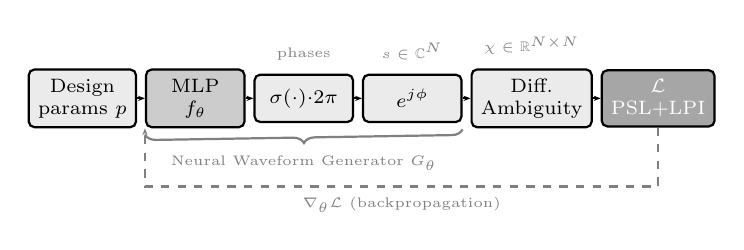
\begin{tikzpicture}[
    node distance=0.3cm and 0.1cm,
    box/.style={draw, rounded corners=2pt, minimum height=0.6cm, minimum width=1.25cm,
                font=\scriptsize, align=center, thick},
    forward/.style={box, fill=black!8},
    neural/.style={box, fill=black!20},
    loss/.style={box, fill=black!35, text=white},
    arrow/.style={-{Stealth[length=2.5pt]}, thick},
    backarrow/.style={-{Stealth[length=2.5pt]}, thick, dashed, gray},
    label/.style={font=\tiny, text=gray},
]
% Forward pass (top row)
\node[forward] (input) {Design\\params $p$};
\node[neural, right=of input] (mlp) {MLP\\$f_\theta$};
\node[forward, right=of mlp] (sigmoid) {$\sigma(\cdot){\cdot}2\pi$};
\node[forward, right=of sigmoid] (exp) {$e^{j\phi}$};
\node[forward, right=of exp] (amb) {Diff.\\Ambiguity};
\node[loss, right=of amb] (loss) {$\mathcal{L}$\\PSL+LPI};

% Arrows forward
\draw[arrow] (input) -- (mlp);
\draw[arrow] (mlp) -- (sigmoid);
\draw[arrow] (sigmoid) -- (exp);
\draw[arrow] (exp) -- (amb);
\draw[arrow] (amb) -- (loss);

% Labels above arrows
\node[label, above=0.05cm of sigmoid] {phases};
\node[label, above=0.05cm of exp] {$s \in \mathbb{C}^N$};
\node[label, above=0.05cm of amb] {$\chi \in \mathbb{R}^{N{\times}N}$};

% Brace for neural network (closer to boxes)
\draw[decorate, decoration={brace, amplitude=4pt, mirror}, thick, gray]
    ($(mlp.south west)+(0,-0.08)$) -- ($(exp.south east)+(0,-0.08)$)
    node[midway, below=5pt, font=\tiny, text=gray] {Neural Waveform Generator $G_\theta$};

% Backprop arrow (further below, clear of brace)
\draw[backarrow] (loss.south) -- ++(0,-0.75) -| node[label, below, pos=0.25] {$\nabla_\theta \mathcal{L}$ (backpropagation)} (mlp.south west);
\end{tikzpicture}
\caption{End-to-end training pipeline. The neural waveform generator is trained by backpropagating radar performance metrics through the differentiable ambiguity function into the network weights.}
\label{fig:pipeline}
\end{figure}

\subsection{Inference}

Once trained, the generator produces waveforms via a single forward pass:
\begin{equation}
s^* = G_\theta(\lambda^*, z^*)
\label{eq:inference}
\end{equation}
for any desired $\lambda^*$ and noise seed $z^*$.
This requires no iterative optimization, no ambiguity function evaluation, and completes in under one millisecond on both CPU and GPU hardware.
Multiple candidates can be generated (using different $z$ values) and the best selected via a single ambiguity function evaluation.

This capability is particularly relevant for cognitive radar~\cite{haykin2006cognitive, gurbuz2019cognitive}, where waveforms must adapt to changing environmental conditions in real time.
The trained generator serves as a learned waveform library that can be queried instantly with any design specification.


% ==============================================================
\section{Experimental Validation}
\label{sec:experiments}

\subsection{Setup}

We validate our approach on the joint optimization of PSL and spectral variance (LPI) for constant-modulus phase-coded waveforms.
All experiments operate on signals $s[n] = e^{j\phi[n]}$ with $\phi[n] \in [0, 2\pi)$.

\textbf{Methods compared:}
\begin{itemize}
    \item \textbf{Gradient, full 2D} (using our differentiable ambiguity function): Adam optimizer on the full two-dimensional ambiguity function, learning rate 0.01, 2000 iterations.
    \item \textbf{Gradient, 1D autocorrelation}: Adam optimizer on the zero-Doppler autocorrelation PSL only, representing the analytical gradient approach where gradients are computed for a specific 1D cost function rather than the full 2D ambiguity surface.
    \item \textbf{Genetic algorithm} (GA): Population size 50, 300 generations, tournament selection with elitism.
    \item \textbf{Neural waveform generator}: MLP with 4 residual blocks, hidden dimension 256, trained for 200 epochs with batch size 32.
\end{itemize}

\textbf{Configurations:}
We test across five trade-off parameters $\lambda \in \{0.0, 0.25, 0.5, 1.0, 2.0\}$ and four waveform lengths $N \in \{64, 128, 256, 512\}$.
While the formulation supports $N$ up to approximately 16{,}384 on current GPUs (Section~\ref{sec:diffambiguity}), we limit experiments to $N \leq 512$ so that the GA baseline remains computationally tractable for fair comparison.
The primary comparison uses $N = 256$, representing realistic medium-range radar pulses (25.6~$\mu$s at 10~MHz sampling).

\textbf{Statistical rigor:}
We report mean $\pm$ standard deviation across multiple independent random seeds for all experiments: 20 seeds for the main gradient-vs-GA comparison, 10 seeds for the baseline and neural generator evaluations, and 5 seeds for ablations and scaling benchmarks.

\textbf{Hardware:}
CPU experiments use an Intel Core i7-1165G7 @ 2.80~GHz.
GPU experiments use an NVIDIA Tesla T4 (16~GB) via Modal cloud compute.

\textbf{Reproducibility:}
Source code is available at \url{https://github.com/marcbara/graf-psl-lpi}.

\subsection{Gradient-Based vs.\ Population-Based Optimization}

We first compare gradient-based optimization (using the differentiable ambiguity function with Adam) against the genetic algorithm baseline.

\subsubsection{Convergence Analysis}

Fig.~\ref{fig:pareto_psl} presents the Pareto frontiers and PSL comparison between both methods across all $\lambda$ values, with error bars from 20 random seeds.

\begin{figure}[!htbp]
\centering
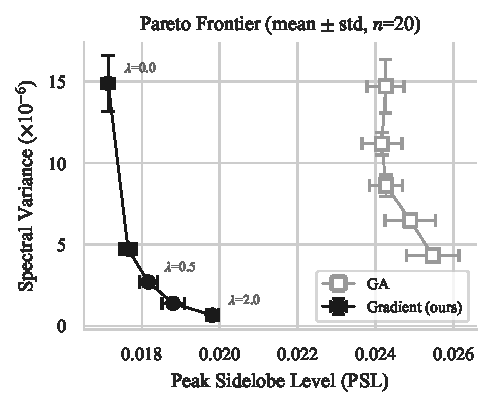
\includegraphics[width=\columnwidth]{fig_pareto.pdf}
\caption{Pareto frontier for gradient-based optimization vs.\ GA ($N=256$, mean $\pm$ std over 20 seeds). The gradient-based solutions consistently dominate GA at every trade-off point.}
\label{fig:pareto_psl}
\end{figure}

\subsubsection{Multi-Objective Performance}

The gradient-based solutions consistently dominate the GA solutions, achieving 2.2--3.0~dB lower PSL at every spectral variance level.
Fig.~\ref{fig:comparison} shows the per-$\lambda$ PSL comparison and computational time.

\begin{figure}[!htbp]
\centering
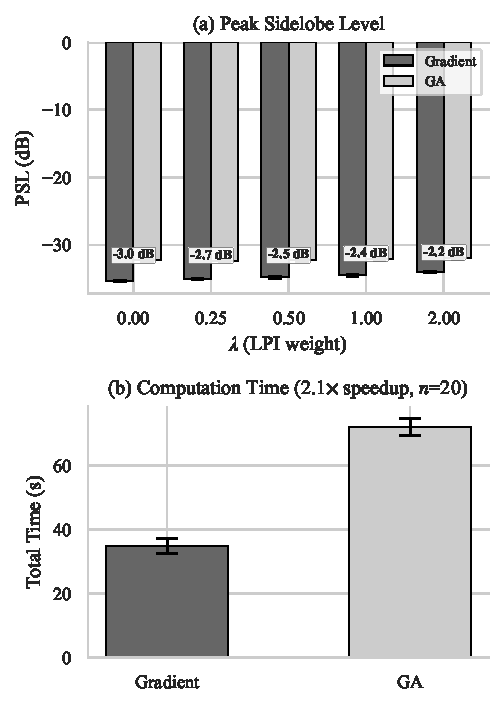
\includegraphics[width=\columnwidth]{fig_psl_comparison.pdf}
\caption{(a) PSL comparison across $\lambda$ values with error bars. (b) Total computation time showing $2.1\times$ speedup. All results over 20 random seeds.}
\label{fig:comparison}
\end{figure}

Table~\ref{tab:results} summarizes the results.

\begin{table}[!htbp]
\centering
\caption{PSL comparison ($N=256$, mean $\pm$ std over 20 seeds, Tesla T4). Total time per method (all 5 $\lambda$ values): Gradient $34.8{\pm}2.3$~s, GA $72.0{\pm}2.6$~s ($2.1\times$ speedup).}
\label{tab:results}
\renewcommand{\arraystretch}{1.1}
\begin{tabular}{@{}cccc@{}}
\toprule
$\lambda$ & \textbf{Gradient (dB)} & \textbf{GA (dB)} & \textbf{$\Delta$ (dB)} \\
\midrule
0.00 & $-35.3{\pm}0.1$ & $-32.3{\pm}0.2$ & $-3.0$ \\
0.25 & $-35.1{\pm}0.1$ & $-32.3{\pm}0.2$ & $-2.7$ \\
0.50 & $-34.8{\pm}0.1$ & $-32.3{\pm}0.2$ & $-2.5$ \\
1.00 & $-34.5{\pm}0.1$ & $-32.1{\pm}0.2$ & $-2.4$ \\
2.00 & $-34.1{\pm}0.1$ & $-31.9{\pm}0.2$ & $-2.2$ \\
\bottomrule
\end{tabular}
\end{table}

\subsection{Full 2D vs.\ 1D Autocorrelation Optimization}

A key advantage of our differentiable ambiguity function is that it optimizes over the \emph{full two-dimensional} delay-Doppler surface, rather than the zero-Doppler autocorrelation alone.
To quantify this advantage, we compare gradient descent on the full 2D ambiguity function (our approach) against gradient descent on the 1D autocorrelation PSL---the type of cost function for which analytical gradients are typically derived in the literature~\cite{song2015optimization, alaee2017coordinate, baden2018multiobjective}.

Table~\ref{tab:baseline} shows the results.
Optimizing the full 2D ambiguity function achieves 7.3~dB lower PSL than the 1D autocorrelation baseline.
The timing advantage ($25\times$) is partly methodological and partly implementational: the matrix-based 2D formulation is inherently more GPU-friendly than the loop-based 1D autocorrelation computation.
A highly optimized 1D implementation (e.g., using the FFT-based $O(N\log N)$ autocorrelation tricks of~\cite{song2015optimization}) would narrow this timing gap, but would not close the 7.3~dB PSL gap, which arises because optimizing the full delay-Doppler surface suppresses sidelobes that the zero-Doppler cut alone cannot address.
The 2D approach also exhibits substantially lower variance across seeds ($\pm 0.1$~dB vs.\ $\pm 0.5$--$1.5$~dB), indicating more consistent convergence.

\begin{table}[!htbp]
\centering
\caption{Full 2D ambiguity vs.\ 1D autocorrelation optimization ($N=256$, 10 seeds).}
\label{tab:baseline}
\renewcommand{\arraystretch}{1.1}
\begin{tabular}{@{}lcccc@{}}
\toprule
 & \multicolumn{2}{c}{\textbf{PSL (dB)}} & \multicolumn{2}{c}{\textbf{Time (s)}} \\
\cmidrule(lr){2-3} \cmidrule(lr){4-5}
\textbf{Method} & $\lambda{=}0$ & $\lambda{=}1$ & mean & std \\
\midrule
1D autocorrelation & $-28.0{\pm}0.5$ & $-27.9{\pm}1.1$ & 476.4 & 5.5 \\
Full 2D (ours)     & $-35.3{\pm}0.1$ & $-34.5{\pm}0.1$ & 19.3  & 0.4 \\
\midrule
\textbf{Improvement} & \textbf{7.3 dB} & \textbf{6.6 dB} & \multicolumn{2}{c}{\textbf{24.7$\times$}} \\
\bottomrule
\end{tabular}
\end{table}

This result indicates that the full 2D formulation finds better waveforms in this setup by jointly optimizing across all delay-Doppler pairs, not just the zero-Doppler cut.
This capability is naturally enabled by the differentiable ambiguity function; achieving comparable results with analytical gradient methods would require deriving new gradient expressions for the full 2D objective---precisely the effort that AD eliminates.

\subsection{Spectral Mask Constraint: Composability}

To demonstrate the composability of the AD-based approach, we add a spectral mask constraint for interference avoidance---a practical radar scenario where the waveform must avoid transmitting in certain frequency bands.

We define a spectral notch centered at 25\% of the bandwidth with 8\% width, and add a penalty term:
\begin{equation}
\mathcal{L}_{\text{mask}} = \sum_k \frac{|S[k]|^2}{\sum_k |S[k]|^2} \cdot M[k]
\label{eq:mask}
\end{equation}
where $M[k] = 1$ in the forbidden band and $0$ elsewhere.
The total loss becomes $\mathcal{L} = \text{PSL} + 0.5 \cdot \alpha \cdot \text{SV} + 5 \cdot \mathcal{L}_{\text{mask}}$.

Adding this constraint required only defining~\eqref{eq:mask} as a differentiable function; no gradient re-derivation was necessary.

Table~\ref{tab:mask} shows the results over 10 seeds.
With the mask constraint, energy in the forbidden band drops from 7.7\% to effectively 0.0\%, at a cost of only 0.2~dB in PSL.
This demonstrates the practical advantage of AD-compatible ambiguity functions: new operational constraints can be incorporated without manual gradient re-derivation.

\begin{table}[!htbp]
\centering
\caption{Spectral mask constraint results ($N=256$, $\lambda=0.5$, 10 seeds).}
\label{tab:mask}
\renewcommand{\arraystretch}{1.1}
\begin{tabular}{@{}lccc@{}}
\toprule
\textbf{Configuration} & \textbf{PSL (dB)} & \textbf{Notch Energy} \\
\midrule
Without mask & $-34.8$ & $7.7\%$ \\
With mask    & $-34.6$ & $< 0.01\%$ \\
\bottomrule
\end{tabular}
\end{table}

\subsection{Downstream Radar Performance}

To assess the operational consequence of improved ambiguity shaping, we simulate matched-filter range-Doppler responses for point-target scenes using the optimized waveforms.
In the point-target scene considered here, the periodic ambiguity function $\chi[k,m]$ corresponds to the matched-filter range-Doppler response of a target at delay~$k$ and Doppler~$m$; for a multi-target scene, the resulting range-Doppler map is the superposition of shifted ambiguity responses weighted by target amplitudes.

\subsubsection{Weak-Target Detection}

We simulate a two-target scene: a strong target at delay-Doppler offset $(20, 30)$ and a weak target at $(40, -20)$ with amplitude $-15$~dB relative to the strong target, embedded in noise at 30~dB SNR.
Table~\ref{tab:detection} summarizes the detection metrics.
The full 2D optimization achieves the highest peak-to-sidelobe ratio (16.5~dB) and the best weak-target visibility (9.1~dB above the sidelobe floor), directly translating the 7.3~dB PSL improvement from Table~\ref{tab:baseline} into improved target separability.
The 1D autocorrelation baseline produces the weakest detection performance (weak target only 5.4~dB above sidelobes), because it suppresses sidelobes only along the zero-Doppler cut while leaving cross-Doppler sidelobes unconstrained.

\begin{table}[!htbp]
\centering
\caption{Detection metrics for a two-target scene ($N=256$, $\lambda=0.5$).}
\label{tab:detection}
\renewcommand{\arraystretch}{1.1}
\begin{tabular}{@{}lccc@{}}
\toprule
\textbf{Method} & \textbf{PSL (dB)} & \textbf{P/SL (dB)} & \textbf{Weak$-$SL (dB)} \\
\midrule
GA                & $-32.2$ & $15.6$ & $8.2$ \\
1D Autocorr.      & $-25.8$ & $12.8$ & $5.4$ \\
Full 2D (ours)    & $-34.8$ & $16.5$ & $9.1$ \\
\bottomrule
\end{tabular}
\end{table}

\subsubsection{Spectral Avoidance}

We extend the spectral-mask experiment from Section~\ref{sec:experiments}-C to show its effect on waveform properties.
Fig.~\ref{fig:interference} compares the power spectra and zero-Doppler ambiguity cuts of waveforms optimized with and without a spectral notch constraint (forbidding transmission in a band centered at 25\% of the bandwidth).
With the mask, energy in the forbidden band drops from 7.7\% to below 0.01\% at a cost of only 0.2~dB in PSL ($-34.8 \rightarrow -34.6$~dB), demonstrating that spectral avoidance can be achieved with negligible impact on ambiguity performance.

\begin{figure}[!htbp]
\centering
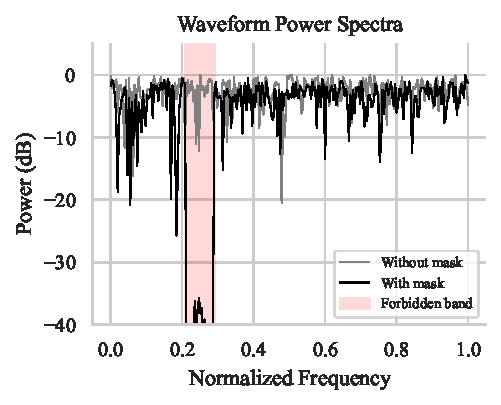
\includegraphics[width=\columnwidth]{fig_interference.pdf}
\caption{Waveform power spectra with and without the spectral mask constraint. The forbidden band (red shading) is fully suppressed at a cost of only 0.2~dB in PSL ($-34.8 \rightarrow -34.6$~dB).}
\label{fig:interference}
\end{figure}

\subsection{Neural Waveform Generator}

\subsubsection{Training}

Fig.~\ref{fig:training} shows the training convergence of the neural waveform generator for $N = 256$.
The network converges within approximately 150 epochs (141~seconds on a Tesla T4 GPU with 10 gradient steps per epoch at batch size 32), after which it can generate waveforms for any $\lambda$ value without further optimization.

\begin{figure}[!htbp]
\centering
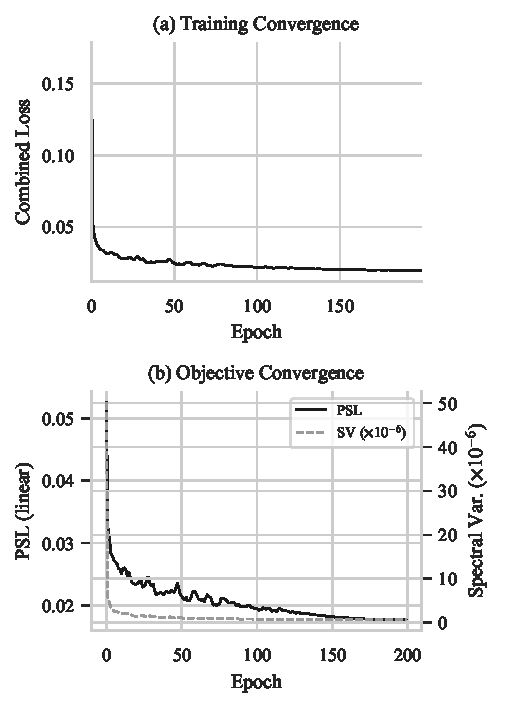
\includegraphics[width=\columnwidth]{fig_neural_training.pdf}
\caption{Neural waveform generator training convergence ($N=256$, Tesla T4). (a) Combined loss. (b) PSL and spectral variance objectives over training epochs.}
\label{fig:training}
\end{figure}

\subsubsection{Generated Waveform Quality}

Table~\ref{tab:neural_results} compares the quality of neural-generated waveforms against iteratively optimized waveforms across $\lambda$ values, with error bars from 10 independent training seeds.
The neural generator achieves PSL within 0.3--1.6~dB of the iterative optimizer.
The gap is expected: the iterative method optimizes each waveform individually for 2000 iterations, while the generator must learn a single mapping that covers the entire $\lambda$ range.
The gap narrows at higher $\lambda$ values, where the spectral variance objective smooths the loss landscape.

\subsubsection{Architecture Ablation}

Table~\ref{tab:ablation} shows the effect of network size and training duration on generated waveform quality, using a reduced training budget (1 gradient step per epoch, batch size 16) to isolate architectural effects.
Under this budget, the medium architecture (128 hidden, 3 layers) achieves the best PSL, suggesting that larger models require more training to realize their capacity.
With the full training schedule (10 steps per epoch, batch size 32), the 256-hidden model achieves $-34.2$~dB (Table~\ref{tab:neural_results}), outperforming the ablation results.
Training for 200 epochs provides approximately 1~dB improvement over 50 epochs across all architectures.

\begin{table}[!htbp]
\centering
\caption{Neural generator ablation ($N=256$, PSL in dB, mean over 5 seeds).}
\label{tab:ablation}
\renewcommand{\arraystretch}{1.1}
\begin{tabular}{@{}lccc@{}}
\toprule
\textbf{Configuration} & \textbf{Params} & $\lambda{=}0$ & $\lambda{=}1$ \\
\midrule
Small (64d, 2L)  & 16{,}960   & $-31.5$ & $-32.4$ \\
Medium (128d, 3L) & 67{,}200   & $-32.6$ & $-33.3$ \\
Full (256d, 4L)   & 332{,}288  & $-31.8$ & $-32.4$ \\
Large (512d, 4L)  & 1{,}188{,}608 & $-30.7$ & $-31.8$ \\
\midrule
Full, 50 epochs          & 332{,}288  & $-30.7$ & $-31.3$ \\
Full, 100 epochs         & 332{,}288  & $-31.4$ & $-31.9$ \\
Full, 200 epochs         & 332{,}288  & $-31.8$ & $-32.4$ \\
\bottomrule
\end{tabular}
\end{table}

\begin{table}[!htbp]
\centering
\caption{Neural generator vs.\ iterative gradient optimization ($N=256$, mean $\pm$ std over 10 seeds for neural, 20 seeds for gradient).}
\label{tab:neural_results}
\renewcommand{\arraystretch}{1.1}
\begin{tabular}{@{}ccc@{}}
\toprule
$\lambda$ & \textbf{Neural PSL (dB)} & \textbf{Gradient PSL (dB)} \\
\midrule
0.00 & $-33.7{\pm}0.1$ & $-35.3{\pm}0.1$ \\
0.25 & $-34.1{\pm}0.1$ & $-35.1{\pm}0.1$ \\
0.50 & $-34.1{\pm}0.1$ & $-34.8{\pm}0.1$ \\
1.00 & $-34.2{\pm}0.1$ & $-34.5{\pm}0.1$ \\
2.00 & $-34.2{\pm}0.1$ & $-34.1{\pm}0.1$ \\
\bottomrule
\end{tabular}
\end{table}

\subsubsection{Inference Speed}

The trained neural generator produces waveforms in a single forward pass.
Table~\ref{tab:timing} compares the time to produce one optimized waveform across all three methods.

\begin{table}[!htbp]
\centering
\caption{Time to produce one optimized waveform ($N=256$, Tesla T4).}
\label{tab:timing}
\renewcommand{\arraystretch}{1.1}
\begin{tabular}{@{}lcc@{}}
\toprule
\textbf{Method} & \textbf{Time} & \textbf{Requires optimization?} \\
\midrule
GA                      & $\sim$14.4 s  & Yes (per waveform) \\
Gradient descent        & $\sim$7.0 s   & Yes (per waveform) \\
Neural generator        & $<$1 ms            & No (single forward pass) \\
\bottomrule
\end{tabular}
\end{table}

The neural generator achieves a ${>}10{,}000\times$ speedup at inference time compared to gradient descent, and ${>}20{,}000\times$ compared to GA.
The one-time training cost (141~seconds) is amortized across all subsequent waveform generation requests---equivalent to optimizing approximately 20 waveforms iteratively.

\subsection{Scaling and GPU Performance}

\subsubsection{Waveform Length Scaling}

Fig.~\ref{fig:scaling} shows computation time and PSL performance as a function of waveform length $N$.
PSL improves by approximately 6~dB per doubling of $N$, consistent with theoretical expectations.

\begin{figure}[!htbp]
\centering
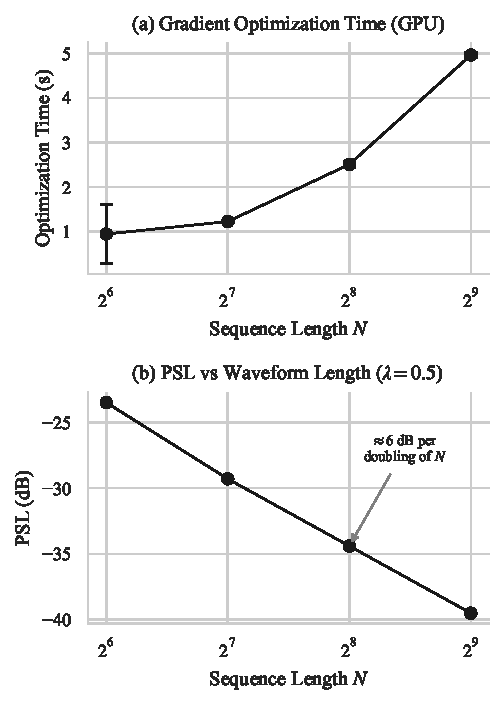
\includegraphics[width=\columnwidth]{fig_n_scaling.pdf}
\caption{Scaling with waveform length $N$ (GPU, $\lambda=0.5$). (a) Optimization time. (b) Achieved PSL, showing ${\approx}6$~dB improvement per doubling of $N$.}
\label{fig:scaling}
\end{figure}

\subsubsection{GPU Acceleration}

Table~\ref{tab:gpu} reports GPU vs.\ CPU performance for the differentiable ambiguity function forward pass.

\begin{table}[!htbp]
\centering
\caption{GPU vs.\ CPU forward pass time (milliseconds).}
\label{tab:gpu}
\renewcommand{\arraystretch}{1.1}
\begin{tabular}{@{}ccccc@{}}
\toprule
$N$ & \textbf{CPU} & \textbf{GPU} & \textbf{Speedup} \\
\midrule
64   & 0.25 & 0.23 & 1.1$\times$ \\
128  & 0.56 & 0.21 & 2.6$\times$ \\
256  & 1.68 & 0.22 & 7.8$\times$ \\
512  & 8.65 & 0.22 & 39.0$\times$ \\
1024 & 32.57 & 0.86 & 37.9$\times$ \\
\bottomrule
\end{tabular}
\end{table}

GPU acceleration provides increasing benefit for larger $N$, as shown in Fig.~\ref{fig:gpu}, with speedups reaching $39\times$ at $N=512$.
The GPU forward pass time remains nearly constant (${\approx}0.2$~ms) up to $N=512$, while CPU time scales quadratically, demonstrating the parallelism of the matrix-based formulation.

\begin{figure}[!htbp]
\centering
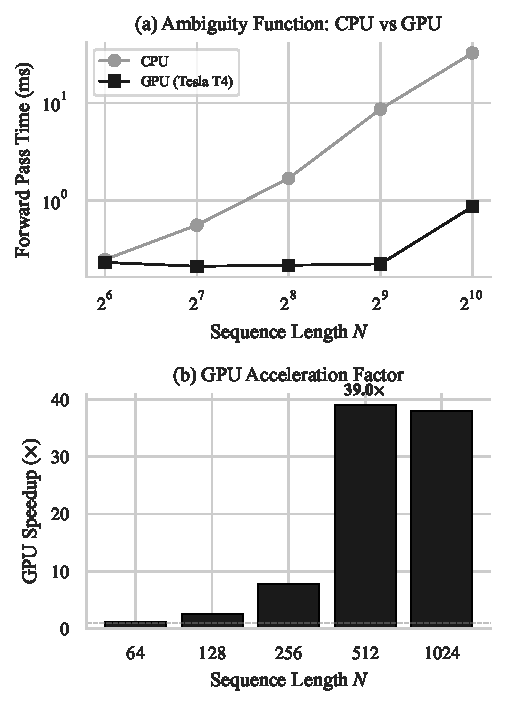
\includegraphics[width=\columnwidth]{fig_gpu_scaling.pdf}
\caption{GPU vs.\ CPU performance for the differentiable ambiguity function forward pass (Tesla T4). (a) Absolute timing. (b) GPU acceleration factor, reaching $39\times$ at $N=512$.}
\label{fig:gpu}
\end{figure}


% ==============================================================
\section{Discussion}
\label{sec:discussion}

\subsection{Practical Implications}

The neural waveform generator supports a practical operating mode for cognitive radar systems.
Rather than running iterative optimization in the radar processing loop---which is computationally prohibitive for real-time adaptation---a pre-trained generator can produce optimized waveforms instantly in response to changing environmental conditions or mission requirements.

The differentiable ambiguity function also benefits traditional iterative optimization workflows.
Adding a new performance metric to the optimization (e.g., Doppler tolerance, spectral mask compliance, interference mitigation) requires only defining the metric as a differentiable function---no gradient re-derivation.
This lowers the barrier for radar engineers to experiment with different multi-objective formulations.

\subsection{Comparison to Analytical Gradient Methods}

We do not claim that our differentiable implementation produces better gradients than the analytical derivations of Alhujaili~et~al.~\cite{alhujaili2020quartic} or Mohr~et~al.~\cite{mohr2021gradient} for their specific problem formulations.
For a fixed objective with known analytical gradients, a specialized implementation may be more computationally efficient, as it avoids the overhead of AD graph construction.
Direct comparison is not straightforward, as these methods address different formulations: QGD~\cite{alhujaili2020quartic} operates on the slow-time ambiguity function under constant modulus constraints on the complex circle manifold, while Mohr~et~al.~\cite{mohr2021gradient} target PCFM waveforms specifically.

Our contribution is \emph{generality} and \emph{composability}.
The analytical methods derive gradients for specific cost functions on specific manifolds; our implementation provides gradients for any differentiable function of the periodic ambiguity surface considered here, and can be composed with upstream neural networks and downstream custom loss terms.
The neural waveform generator is the clearest demonstration of this composability: reproducing the same end-to-end training workflow with analytical methods would require deriving and maintaining gradients through the full ambiguity computation for each new upstream parameterization.

\subsection{Limitations}

\textbf{Periodic assumption.}
Our formulation computes the periodic (circular) ambiguity function, appropriate for phase-coded waveforms but not directly applicable to all waveform types.
Extension to aperiodic formulations requires alternative correlation computation strategies while maintaining differentiability.

\textbf{Memory scaling.}
The $O(N^2)$ memory requirement for the circulant shift matrix scales quadratically; however, even $N = 16{,}384$ requires only ${\sim}6$~GB with gradient buffers, which is practical on current GPUs.
For significantly longer waveforms, block-based or sparse formulations could reduce memory usage.

\textbf{Generator generalization.}
The neural generator's quality is bounded by its training distribution.
Extrapolation beyond the training range of $\lambda$ values may degrade performance.
However, retraining with an expanded range is straightforward given the differentiable pipeline.

\textbf{Baseline scope.}
We compare against GA as the multi-objective baseline rather than reimplementing the specific gradient methods of~\cite{alhujaili2020quartic} or~\cite{mohr2021gradient}, as those address different problem formulations (slow-time ambiguity shaping and PCFM waveforms, respectively) that are not directly comparable to our phase-coded PSL/LPI setup.

\subsection{Future Work}

All experiments in this work are simulation-based.
Hardware-in-the-loop validation---measuring the actual ambiguity function of generated waveforms on a software-defined radio (SDR) testbed---would further strengthen the practical claims and is a natural next step enabled by the open-source implementation.

Other extensions include cross-ambiguity functions for MIMO radar, more expressive generator architectures (e.g., conditional transformers), integration with full radar signal processing chains for end-to-end system optimization, and deployment on embedded radar platforms with fixed-point constraints.


% ==============================================================
\section{Conclusion}
\label{sec:conclusion}

We have presented a practical AD-compatible formulation of the periodic radar ambiguity function and shown that it enables both flexible full-2D waveform optimization and end-to-end neural waveform generation.
The formulation uses parallelized FFT operations with proper Wirtinger derivative handling, achieving $O(N^2 \log N)$ complexity while maintaining mathematical equivalence to the standard periodic ambiguity function.

We demonstrated two applications of this differentiable implementation:
(i) gradient-based optimization on the full 2D ambiguity function, achieving 2.2--3.0~dB PSL improvement over GA and 7.3~dB over 1D autocorrelation baselines;
(ii) extensibility to new constraints without gradient re-derivation, demonstrated by adding a spectral mask objective; and
(iii) a neural waveform generator that, once trained in approximately 141~seconds on GPU, produces optimized waveforms (within 0.3--1.6~dB of iterative optimization) for any design specification in under one millisecond---a capability enabled by the AD-compatible ambiguity function.

The implementation is open-source, GPU-accelerated, and compatible with standard deep learning frameworks, providing a bridge between classical radar signal processing and modern machine learning.


% ==============================================================
\section*{Acknowledgment}
GPU experiments were conducted using Modal cloud compute.

\textbf{AI Disclosure:} An AI assistant (Claude, Anthropic) was used during the preparation of this manuscript for code development assistance, LaTeX editing, and prose refinement.
All technical content, experimental design, and scientific conclusions are the sole responsibility of the author.
The AI system was not used to generate figures, experimental results, or mathematical derivations.


\bibliographystyle{IEEEtran}
\bibliography{references}

\end{document}
